\documentclass[a4paper,12pt]{ctexart}

\usepackage{geometry}
\usepackage{booktabs}
\usepackage{graphicx}
\usepackage[final]{pdfpages}
\usepackage[stable]{footmisc}
\usepackage{threeparttable}
\usepackage{indentfirst}
\usepackage{minted}
\usepackage{listings}
\usepackage{xcolor}
\usepackage{subfigure}
\usepackage{amsmath}
\usepackage{amsfonts}

% \setlength{\parindent}{0pt}
\geometry{top=20mm,bottom=20mm,left=15mm,right=15mm}
\lstset{
    rulesepcolor= \color{gray},
    breaklines=true,
    numbers=left,
    numberstyle= \small,
    commentstyle=\color{gray},
    frame=shadowbox
}


\title{Y23T2W3 例行周报}
\author{杜睿}
% \date{}

\begin{document}
\tableofcontents
\maketitle

\begin{abstract}
    本周对童咏昕TKDD2021的双边在线匹配\cite{8897719}中提到的四种算法进行了复现。
\end{abstract}

\section{论文重述}

离线场景下,任务和工人事先已知;在线场景下,任务或工人突然冒出。众包应用中,任务和工人不是离线资源无法事先已知,因此,这是一个“双边”在线问题。

\begin{enumerate}
    \item 对于离线问题,通常采用线性规划、匈牙利算法求解;引入$X_{i, j}$零一变量(代表是否要将第$i$个工人分配给第$j$个工人)后,问题约束静态(一名工人只能做一个任务,一个任务只能分配给一名工人)、目标单一(最大化收益)。
    \item 对于在线问题,由于缺乏未来全局信息,算法的正确性无法保证;为了参考衡量算法优劣,通常是“事后诸葛亮”,考虑在线情境的解与离线情景最优解的比(竞争比)。竞争比的理论分析一般要考虑最差情况,即对于所有可能的测试用例而言,某种算法获得的\emph{最小竞争比}。
\end{enumerate}

而本论文提出,日常生活中非常极端的最差的测试用例出现概率很低,因此理论分析、数学推导,不一定可以落地生产实际,不能一棒子打死贪心算法:由此提出也要在平均情况下进行分析。

\section{算法复现}

\begin{description}
    \item [顶点] 具有到达时间、消失时间、二维位置、匹配容量和已匹配数四种属性。
    \item [工人] 一类顶点,额外具有标识,可操控范围、成功率3种属性。
    \item [任务] 一类顶点,额外具有标识,完成收益2种属性。
\end{description}

任务和工人的关系存在:
\begin{enumerate}
    \item 能否把某任务匹配给某工人(记作$f$),要考虑4类约束,这涉及已匹配数与匹配容量的限制、二维位置距离与可操控范围的限制、到达时间与消失时间的限制。
    \item 倘若把某任务匹配给某工人,可以获得收益(完成收益与成功率的乘积,记作$g$)。
\end{enumerate}

我们可以考虑将任务和工人的关系用一个二维数组表示,$A_{i, j} = f(i, j) * g(i, j)$。如果取值为零,说明不允许为第$i$名工人分配第$j$项任务;否则,代表试分配后的收益。每次分配后,由于容量发生变化,需要对效益值进行更新。

此外,论文对该问题添加了如下假设:

\begin{enumerate}
    \item 为了简化一个工人可以胜任多项任务的情况,论文将1个$c_w$容量的工人,等价的视作$c_w$个1容量的工人。
    \item 随着时间的推移,某些工人/任务已经消失,也可以更新效益矩阵(算法4)。
    \item 虽然具体的工人和任务信息无法事先了解,但是,工人总数、任务总数、工人的总体容量是可以从历史记录知悉。
\end{enumerate}


下面对每个算法的思想进行简要概述:
\begin{description}
    \item[算法一] 基于随机阈值。对于新到达的顶点,考虑可以与该顶点匹配且收益大于阈值的顶点集,若存在,则随机抽取进行匹配。
    \item[算法二] 受秘书问题启发,将问题分为两个阶段求解。到达顶点不足总顶点的一半时,对新到达顶点,如果可以匹配,就匹配收益最大的;否则,对于新到达的顶点,使用匈牙利算法在目前的效率矩阵上运行,如果新到达的顶点在最优解上被匹配,就进行匹配。
    \item[算法三] 在算法二的基础上进行改进,将第二阶段换做在效率矩阵上重复寻找最大效益进行匹配的贪心策略,以节省运行时间。
    \item[算法四] 在算法三的基础上进行改进,对于已经消失的顶点,更新效率矩阵。  
\end{description}

\section{实验结果}

对于四个算法,在虚拟数据集39个测试样例上进行测试。运行概览如图所示:
\begin{figure}[htbp]
    \centering
    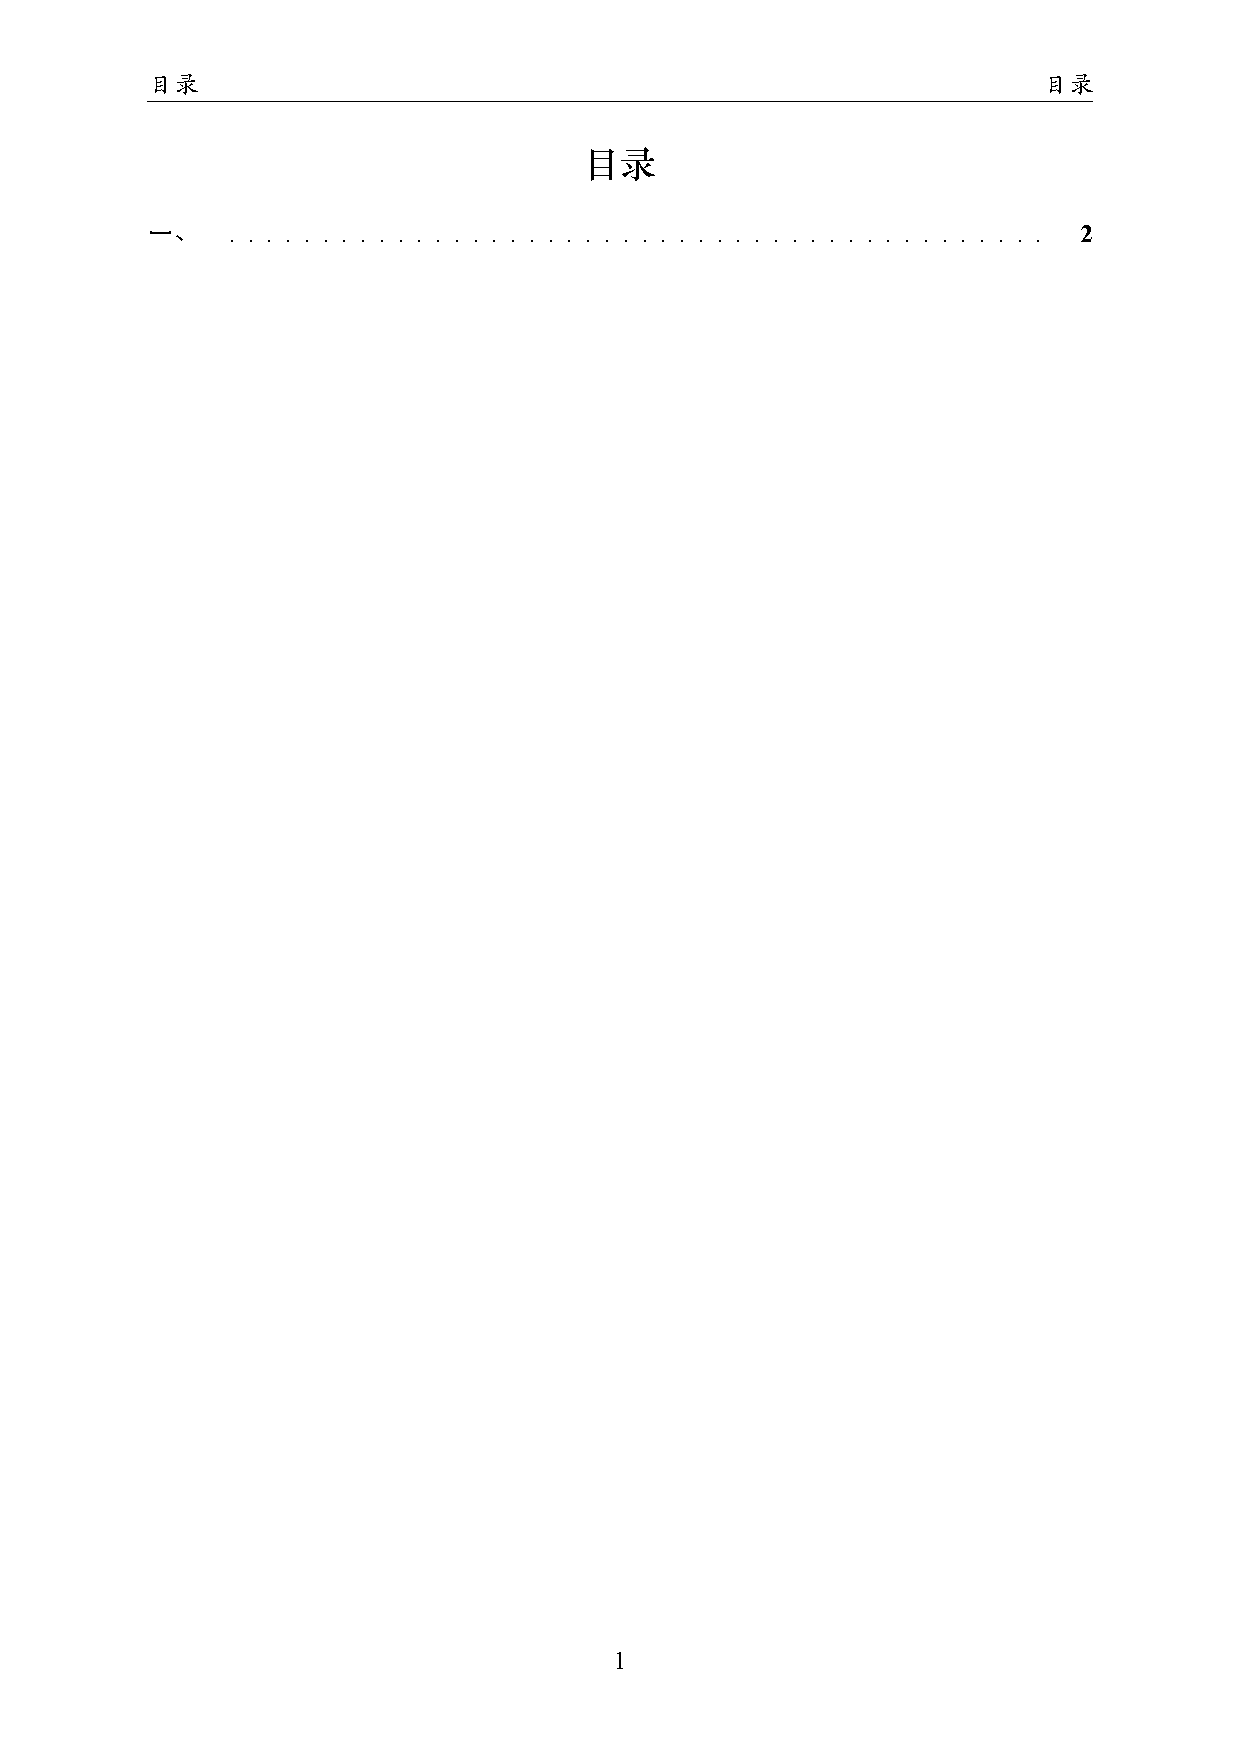
\includegraphics[width=0.76\linewidth]{../main.pdf}
    \caption{实验结果}
\end{figure}

\section{评价与规划}

本周仅对算法伪代码部分进行了复现,在数据集上可以简单跑通;与作者的实验结果效果图存在差异,但暂未进行结果分析和详细比较。下周继续精读该论文,并了解有关拍卖理论的相关知识。

\bibliography{main}
\bibliographystyle{ieeetr}

\end{document}

% \begin{table}[htbp]
%     \caption{常用的处理机调度策略}
%     \centering

%     \begin{threeparttable}
%         \begin{tabular}{cccccc}
%             \toprule
%             算法名称           & 主要适用范围       & 默认调度方式         \\
%             \midrule
%             先来先服务         & 作业调度\&进程调度 & 非抢占式             \\
%             短作业(进程)优先 & 作业调度\&进程调度 & 非抢占式             \\
%             高响应比优先       & 作业调度           & 非抢占式             \\
%             时间片轮转         & 进程调度           & 抢占式(不抢时间片) \\
%             多级反馈队列       & 进程调度           & 抢占式(抢占时间片) \\
%             \bottomrule
%         \end{tabular}

%         \zihao{-6}
%         \begin{tablenotes}
%             \item [*]   调度策略也就是调度算法
%         \end{tablenotes}

%     \end{threeparttable}
%     \qquad
% \end{table}

% \begin{figure}[htbp]
%     \centering
%     \includegraphics[height=550pt]{v1-class-compat.png}
%     \caption{UML类图(第二版)}
% \end{figure}

% \begin{minted}[mathescape,
%     linenos,
%     numbersep=5pt,
%     frame=lines,
%     gobble=4,
%     framesep=2mm]{Java}
%     public interface Observable {
%         void attachObserver(Observer o);

%         void detachObserver(Observer o);

%         void notifyObservers();
%     }
% \end{minted}

% \begin{lstlisting}[language={java},caption={收容队列(基于响应比的优先队列)}]
% private PriorityQueue<Task> queue = new PriorityQueue<>(new Comparator<Task>() {
%     @Override
%     public int compare(Task o1, Task o2) {
%         return (o2.getResponseRate(Clock.minutes) - o1.getResponseRate(Clock.minutes) > 0) ? (1) : (-1);
%     }
% });
% \end{lstlisting}
